\clearpage
\begingroup
\clubpenalty=10000 \widowpenalty=10000 \displaywidowpenalty=10000
\section{方式三：基于RGB-D的目标跟随与自主避障}\label{sec:follow3}
% Reorganized from the supplied Word report; original image bytes and measured data are retained.

本组面向TonyPi抱物穿越挡板赛道的协同任务，实现由后车自身RGB-D观测驱动的目标跟随与自主避障。系统以深度几何和固定外观确认目标，利用头腿局部结构、红块关联及短时光流适应携物与侧身姿态，再通过滚动障碍地图、可达跟随点和导航控制形成执行闭环。本次正式比赛完成，现场确认耗时180秒；以下分别说明方案原理、模块实验、规划回放和比赛证据。


\FloatBarrier
\Needspace{8\baselineskip}
\subsection{实验任务与系统架构}\label{sec:f3-system}
\Needspace{5\baselineskip}
\subsubsection{任务场景与观测边界}
课程综合任务由 TonyPi 携物穿越障碍场地、Turtlebot2 采用不同方式跟随和系统方案交付组成。本组重点实现方式三，即后车依赖自身 RGB-D 感知识别前方机器人，实时生成跟随目标并处理行进路线上的障碍。TonyPi 抱物、步行和转向构成被跟随目标的运动条件；本节重点讨论后车如何从当前观测建立可执行的跟随与避障闭环。

该方法以 RGB、配准深度及本车里程计作为主要输入，不要求前车广播目标位姿。比赛场地中可见的 AR 标签和其他小组机器人属于联合实验环境；方式三对 TonyPi 的身份识别不以标签 ID 为输入。系统也保留前车为 Turtlebot 时的独立目标配置，便于分阶段调试。

图~\ref{fig:f3-01} 展示了室内连续挡板赛道。挡板既限定了可通行走廊，也在拐角形成局部遮挡，后车需同时调整位置、朝向和与前车的间隔。长直通道有利于稳定接近，转弯区则要求机器人及时选择新的行进方向；直接朝目标位置运动容易产生横切弯角或停车点不可达的问题。照片没有可用于可靠测量的统一比例，因此场地总长和通道宽度不由透视图估算。

赛道附近的人员、桌椅、笔记本和线缆增加了背景纹理及深度干扰。TonyPi 抱持红色物块时，胸部颜色与手臂轮廓改变；转成侧身后可见宽度减小，步行时头部、躯干和腿部又有周期性相对摆动。这要求检测器兼顾姿态变化与身份区分，跟踪器也要容忍测量扰动并限制错误关联。

\begin{figure}[H]
\centering
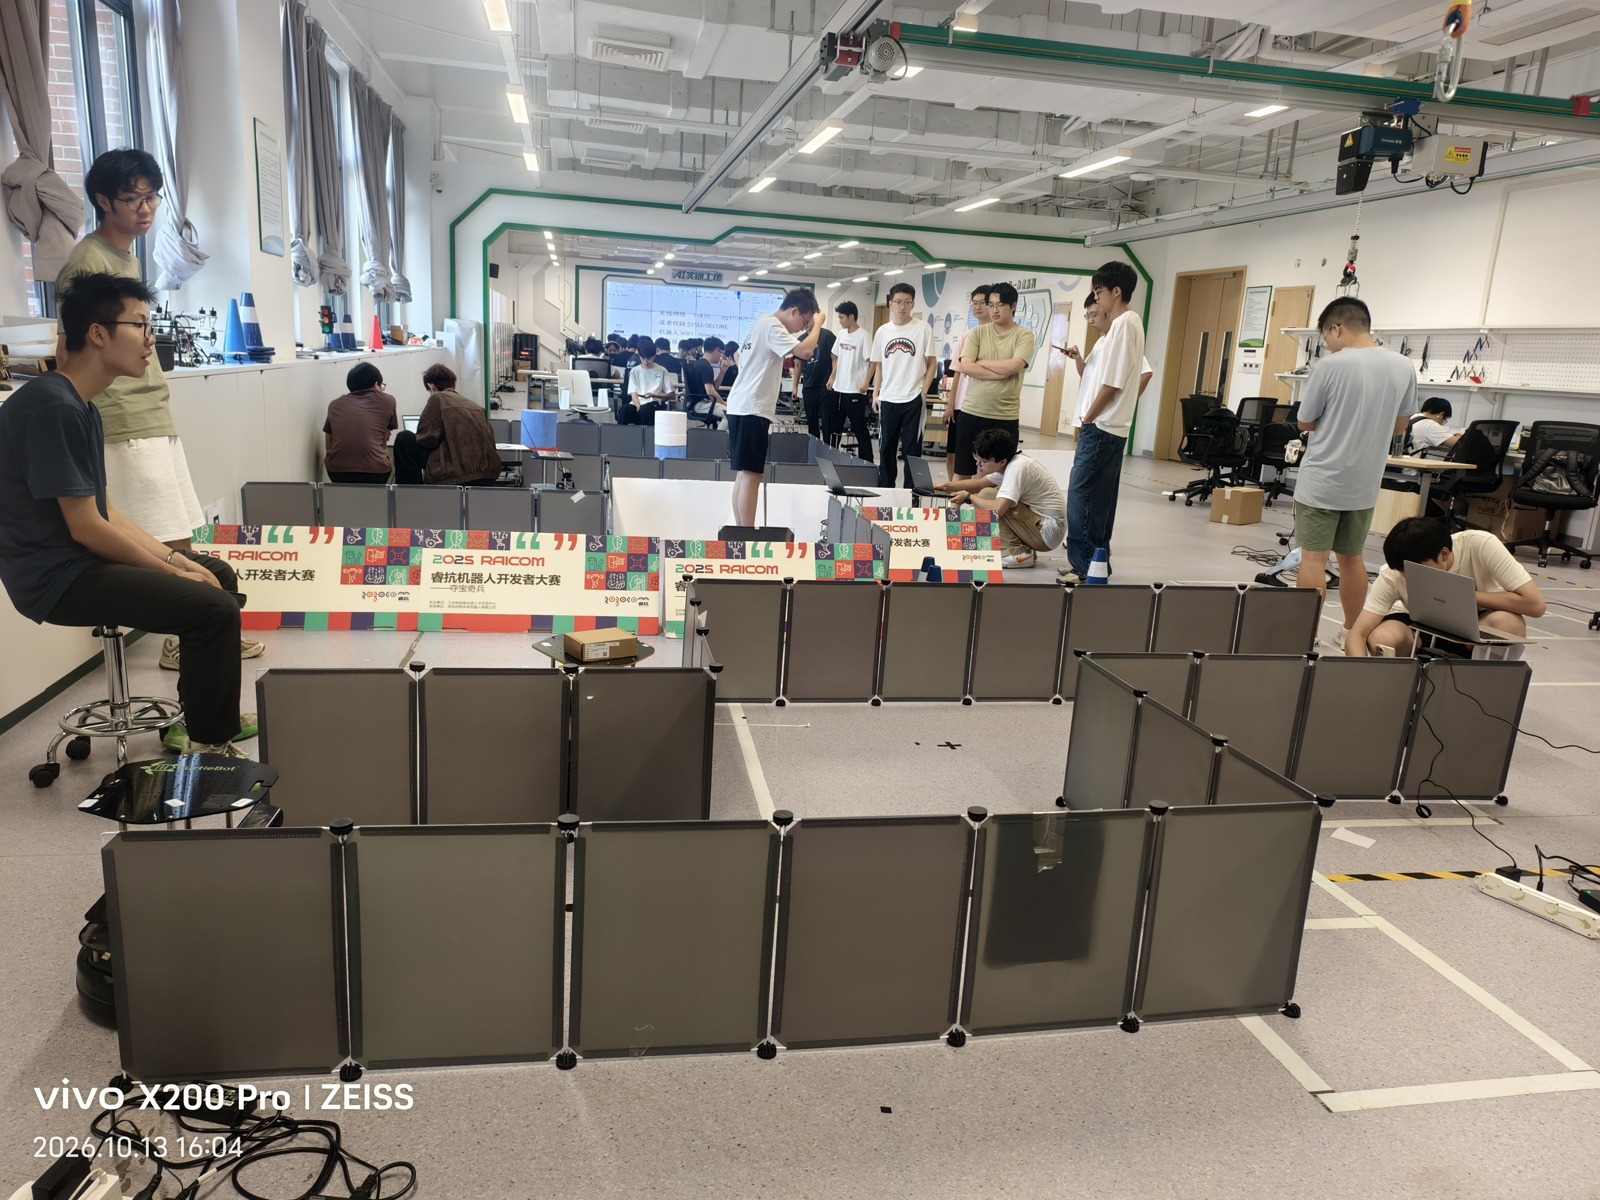
\includegraphics[width=.96\linewidth,height=.36\textheight,keepaspectratio]{figures/follow3/f3_01_site.jpg}
\caption{正式比赛挡板赛道与转弯区域}\label{fig:f3-01}
\end{figure}
\Needspace{16\baselineskip}
\subsubsection{实验平台与数据流}
\begin{table}[H]
\centering\small
\caption{实验平台与运行环境}\label{tab:f3-platform}
\begin{tabularx}{\linewidth}{p{.23\linewidth}Y}\toprule
组成 & 实验配置\\
\midrule
前车 & TonyPi 人形机器人  抱持红色方块行走\\
后车 & Turtlebot2  Kobuki 差速底盘\\
视觉传感器 & Microsoft Kinect  RGB 与配准深度\\
软件环境 & Ubuntu 16.04  ROS Kinetic  Python 2.7  OpenCV\\
计算与显示 & 笔记本及 VMware Ubuntu  目标预览与 RViz\\
任务结果 & 已完成比赛  比赛耗时 180 s\\
\bottomrule\end{tabularx}
\end{table}

比赛视频文件时长为 184.81 秒，共 5556 帧，分辨率为 1920 $\times$ 1080。视频覆盖了现场行进和操作画面；正式比赛耗时采用现场确认的 180 秒，录像时长不直接代替比赛计时。

系统采用感知、地图、规划和执行分层结构。目标检测与场景障碍处理并行读取当前 RGB-D 观测；目标位置经相机内参与 TF 变换进入本车 odom 坐标系，避免后车自身转动时把图像中的横向变化全部解释为前车运动。跟随控制根据时序目标和代价地图选择可执行目标，底盘输出经过独立速度门控。

\begin{figure}[!htbp]
\centering
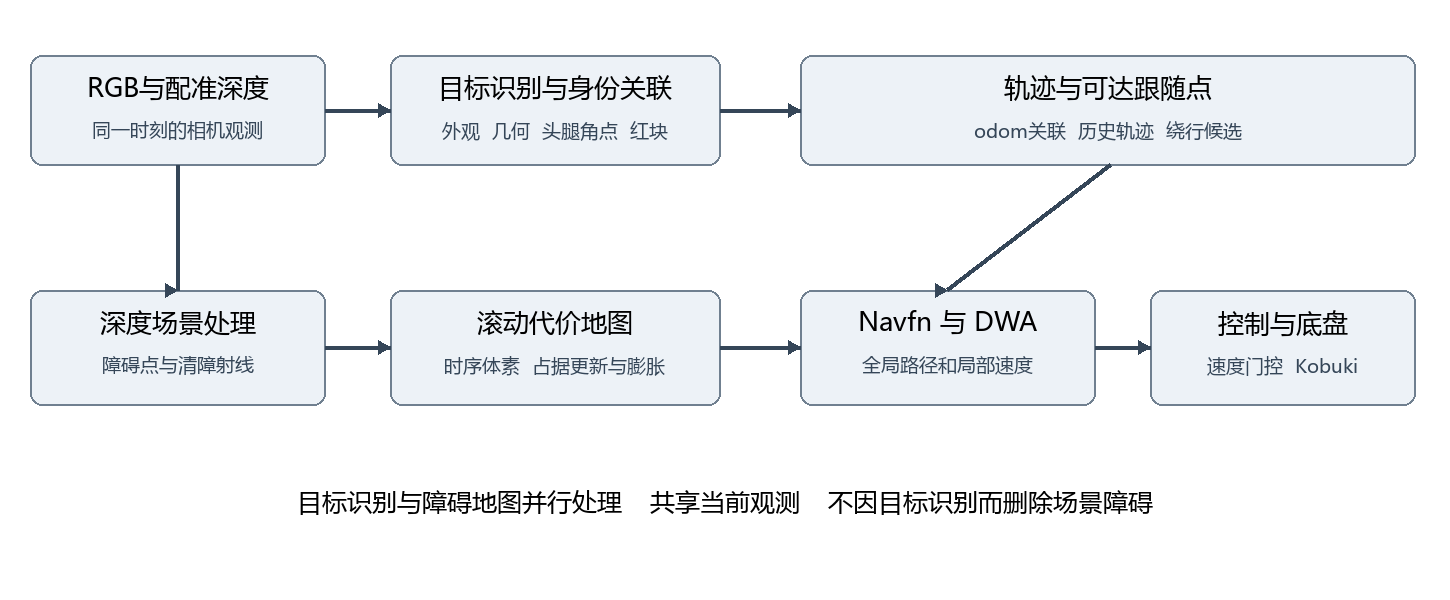
\includegraphics[width=.96\linewidth,height=.36\textheight,keepaspectratio]{figures/follow3/f3_02_dataflow.png}
\caption{方式三视觉跟随与避障数据流}\label{fig:f3-02}
\end{figure}
\Needspace{5\baselineskip}
\subsubsection{观测时效与运行会话}
系统同时记录 RGB、深度和 CameraInfo 的源时间戳，区分传感器采集时间与程序接收时间。最新帧通道和有界同步减少了积压旧帧的问题；检测和障碍处理分开，使较复杂的身份判断不必拖慢点云更新。诊断输出记录检测耗时、观测年龄和地图状态，便于定位停顿发生在输入、识别、规划还是执行层。

场地入口统一启动传感器、识别、导航、预览、RViz 和遥测记录，运动控制使用独占会话管理。Ctrl+C 进入统一退出流程，减少残留同名 ROS 节点影响后续启动。每轮保存生成后的配置和状态日志，使“设定了什么参数”和“最终实际运行了什么参数”能够对应。



\FloatBarrier
\Needspace{8\baselineskip}
\subsection{RGB-D定位与携物身份识别}\label{sec:f3-perception}
\Needspace{5\baselineskip}
\subsubsection{三维测量与坐标统一}
目标定位首先将已校正、且与深度图配准一致的像素恢复为三维点。设目标像素为$(u,v)$，有效深度为$Z$，则相机光学坐标系中的点$\mathbf p_c$及其在本车里程计坐标系中的位置$\mathbf p_o$满足
\begin{equation}\label{eq:f3-projection}
\begin{aligned}
\mathbf p_c & = Z
\begin{bmatrix}
(u-c_x)/f_x & (v-c_y)/f_y & 1
\end{bmatrix}^{\mathsf T},\\
\mathbf p_o(t) & = \mathbf R_{oc}(t)\,\mathbf p_c+\mathbf t_{oc}(t).
\end{aligned}
\end{equation}
其中，$f_x,f_y$为焦距，$c_x,c_y$为主点坐标；$\mathbf R_{oc}(t)$与$\mathbf t_{oc}(t)$为观测时刻从相机光学坐标系到odom坐标系的旋转和平移，由相机安装关系及本车位姿共同确定。跟踪和路径规划使用$\mathbf p_o$的水平位置分量，从而减小后车转动对目标运动判断的影响。

\Needspace{4\baselineskip}
式~\eqref{eq:f3-projection}中的$Z$来自候选区域内的有效深度及聚类支持，零值、非有限数和超量程像素不参与测距。安装位置或朝向变化后，需要重新核对外参；仅有图像检测框不能替代可信的空间位置。

\Needspace{5\baselineskip}
\subsubsection{深度候选与头腿结构验证}
TonyPi 检测首先利用地面模型和深度分层生成有物理尺度的候选。候选经过尺寸、有效深度支持及脚部接地条件筛选，再与登记的多视角外观参考比较。描述符包含颜色分布和轮廓信息；差异分数越低代表越相似，不能将该分数直接解读为神经网络的概率置信度。对共享深度支撑的重叠候选进行抑制，可减少同一机器人产生多个局部框。

整身模板容易受到抱物动作影响，因此我们增加头部和腿脚区域的局部验证。OpenCV \code{goodFeaturesToTrack} 提取 Shi--Tomasi 角点，头部与腿部各保留最多 20 个，胸前、手臂和携物区域不作为稳定角点的主要来源。有效候选至少需要上部 2 个、腿部 4 个角点，并结合固定腿部描述符和实测身高约束。蓝点表示图像角点，而非经过学习得到的机器人关节位置。

侧身时身体变窄，左右腿分区随视角改变。侧身分支对腿部左右区域进行汇合比较，在保留身高和几何一致性的同时降低视角变化造成的描述差异。TonyPi 候选采样步长由 4 像素加密为 2 像素，最低可见宽度允许到 6 cm；这些是候选生成设置，最终仍需外观与结构证据共同通过。
\Needspace{5\baselineskip}
\subsubsection{红块关联与评分调整}
比赛中TonyPi持续抱持红色方块，红块因此可以提供与任务相关的辅助身份证据。该证据只作用于已通过头腿结构及几何检查的候选。以$S_{\mathrm{parts}}$表示原部件差异分数，可将报告中的固定加分规则概括为
\begin{equation}\label{eq:f3-red-score}
S_{\mathrm{adj}}=S_{\mathrm{parts}}-0.10\,\mathbf 1_{\mathcal R}.
\end{equation}
$\mathbf 1_{\mathcal R}$为关联条件的指示量：紧凑红色区域位于候选上身附近，具有有效深度，且红块与身体的深度差不超过$0.18\,\mathrm m$时取1，否则取0。差异分数越小表示越匹配，因此减去0.10会增强已有候选的证据，但红块单独出现不会建立机器人身份。该式是固定规则的记号化表达，不代表学习得到的概率模型。

关联成立时，侧身部件差异的可接受门限可使用0.30；未关联红块时仍限制在0.24。现场采样还表明，RGB与深度边缘偏差、轻微模糊会让红块附近少量非红像素连入身体，造成候选框向上拉长。为此在识别掩膜中增加有界的2像素边缘处理；该处理只影响身份特征，原始障碍深度继续进入地图。




\FloatBarrier
\Needspace{8\baselineskip}
\subsection{时序关联与短时光流补接}\label{sec:f3-tracking}
\Needspace{5\baselineskip}
\subsubsection{位移门限与身份连续性}
每帧候选经过身份检查后，还需要与已有目标在odom平面中的历史位置关联。设当前候选位置为$\mathbf p_t$，上一次有效关联的位置为$\mathbf p_{\mathrm{last}}$，时间差为$\Delta t=t-t_{\mathrm{last}}\geq0$，则位置关联条件写为
\begin{equation}\label{eq:f3-association}
\left\|\mathbf p_t-\mathbf p_{\mathrm{last}}\right\|_2
\leq \min\!\left(r_{\max},\,r_{\mathrm{jitter}}+v_{\max}\Delta t\right).
\end{equation}
$r_{\mathrm{jitter}}$容忍测量抖动，$v_{\max}$限定合理的目标运动范围，$r_{\max}$限制当前关联模式下的最大搜索半径。该条件只提供空间约束，不能替代外观、结构和连续观测确认；多个候选证据接近时保留歧义状态，异常跳变不直接更新目标。

预览中的绿色框表示已完成时序关联的目标，黄色框表示尚未被确认选中的候选。候选框反复变化时，需要结合差异分数、拒绝原因和跟踪状态判断其来源，而不是通过更改显示颜色消除异常。

\Needspace{5\baselineskip}
\subsubsection{光流匹配与补接有效期}
完整检测可能因步态摆动或轻微模糊而短暂失败。程序从已确认目标的头腿角点出发，通过金字塔Lucas--Kanade光流寻找下一帧对应位置，其局部匹配目标可表示为
\begin{equation}\label{eq:f3-lk}
\mathbf d^{*}=\arg\min_{\mathbf d}
\sum_{\mathbf q\in W}
\left[I_t(\mathbf q+\mathbf d)-I_{t-1}(\mathbf q)\right]^2.
\end{equation}
其中，$I_{t-1}$与$I_t$为相邻帧的灰度图像，$W$为角点邻域，$\mathbf d$为图像位移。式~\eqref{eq:f3-lk}描述局部亮度一致性目标，程序调用OpenCV的金字塔光流实现进行迭代求解，并通过前向、反向匹配检查对应关系。\cite{f3-lk-foundation}

图像对应点仍须通过当前深度、点的分布和运动一致性检查。程序最多保留40个角点，短时补接最长为0.22秒，且从原始有效检测时刻计时，不以每次光流输出重新续期。检测恢复后，由真实RGB-D候选继续修正关联。

当多个候选竞争时，光流点落入候选框的比例、候选深度与位置共同参与消歧；只有一个候选明显获得更多支持时才采用该证据。若可靠点不足、当前深度无效或发生明显前景遮挡，则不生成补接观测。

\Needspace{5\baselineskip}
\subsubsection{异常恢复与计算开销}
识别层针对图像位移、模糊与深度缺失保持短时连续性；会话层针对输入超时和底盘数据异常记录具体原因。短暂停顿先停止当前运动输出，并等待新观测恢复后继续原会话，减少一次短时扰动直接结束任务的问题。真实设备断流仍会限制可用信息，软件恢复不能替代传感器与 USB 链路的稳定性。

算法主要由采样深度几何、固定外观比较、有限角点和稀疏光流组成，没有在现场训练深度网络或强化学习模型。单帧深度采样、候选数量和角点预算都有界，因而适合实验中的虚拟机计算条件。12 帧侧身样本的派生扰动回放中，检测耗时中位数约为 46.1--49.4 ms；该值是开发机离线检测时间，不包含 ROS 传输、地图更新和底盘响应。



\FloatBarrier
\Needspace{8\baselineskip}
\subsection{滚动地图与自主避障}\label{sec:f3-navigation}
\Needspace{5\baselineskip}
\subsubsection{身份判断与障碍证据更新}
机器人身份与场景可通行性分别判断。识别到 TonyPi 后，控制器保持跟随间隔；挡板、人员和其他深度物体继续影响规划。即使一个物体不属于目标候选，它仍可能是障碍。这样既避免把红色物体都当目标，也避免通过删掉目标框附近的点来制造虚假的通路。

配准深度经相机内参和坐标变换形成场景点。地图处理将可用于标记障碍的点云与清障射线端点分开：障碍点用于写入占据证据，真实背景和地面回波形成可见空间射线，用于释放射线穿过的旧体素。无效深度不能直接变成最大量程空闲射线；地面回波也不能无条件抹去更高处的障碍。

调试中一度出现重新启动后才能前进的现象。通过采样发现，点云输入本身已接近实时，主要问题是转弯后旧占据点离开视野或落入深度空洞，缺少后续清障射线。为此实现 \code{TemporalVoxelLayer}，在保留三维射线规则的基础上记录原观测时间，并对历史占据证据设置有限记忆。默认障碍记忆为 2 秒，重复旧消息不会续期，观测失效时也不会通过清空地图放行。
\Needspace{5\baselineskip}
\subsubsection{历史轨迹与可达跟随点}
跟随目标应优先依据前车实际走过的路线生成，以减小弯道中直接朝目标中心运动所造成的横切。将当前保留的目标历史折线按弧长参数化为$\boldsymbol\gamma_t(s)$，总长度记为$L_t$，期望跟随间隔记为$d_f$。当历史长度足够，即$L_t\geq d_f$时，名义跟随点为
\begin{equation}\label{eq:f3-standoff}
\mathbf g_t^{\mathrm{nom}}=\boldsymbol\gamma_t(L_t-d_f).
\end{equation}
曲线与跟随点均位于odom平面坐标系。式~\eqref{eq:f3-standoff}沿目标走过的路径回退$d_f$，因此约束的是路径弧长间隔，而非仅保持直线距离。历史不足时，系统按当前目标生成保持间隔的候选，再进行后续可达性检查。

名义点不直接等同于最终导航目标。候选仍需结合车体足迹、栅格连通性、路径长度、软障碍代价、间距误差与方向代价评分；目标附近不可通行时，可以选择绕行子目标。通过弯道或退出局部死角可能需要先侧向运动或阶段性远离目标，不能要求每一步都缩短欧氏距离。失败记录与重试预算用于减少重复选择无效目标；接近子目标时及时更新路径和朝向，以减轻反复减速与对齐。

\Needspace{5\baselineskip}
\subsubsection{Navfn与DWA的规划控制分工}
Navfn在滚动代价地图上生成参考路径，DWA在当前速度和加速度约束内采样线速度$v$与角速度$\omega$，前向模拟对应轨迹$\tau(v,\omega)$。将满足运动限制、足迹碰撞检查及其他有效性条件的候选速度集合记为$\mathcal V_{\mathrm{valid}}$，则选择过程可概括为
\begin{equation}\label{eq:f3-dwa}
(v^{*},\omega^{*})=
\arg\min_{(v,\omega)\in\mathcal V_{\mathrm{valid}}}
\sum_{j} w_j\,C_j\!\left(\tau(v,\omega)\right).
\end{equation}
$C_j$表示路径偏离、目标距离、障碍、朝向等轨迹评价项，$w_j$为运行配置对应的评分尺度。该式描述ROS实现中的多项轨迹评分；无效轨迹先被拒绝，权重及启用项以实际配置为准。\cite{f3-dwa-foundation} 若没有可行候选，则不产生可执行的前进轨迹，交由会话恢复与重规划逻辑处理。

差速底盘的前向模拟满足$\dot{x}=v\cos\theta$、$\dot{y}=v\sin\theta$、$\dot{\theta}=\omega$，其中$\theta$为底盘朝向；当$\omega\ne0$时，转弯半径为$R=|v/\omega|$。合理分配线速度与角速度，并检查完整足迹扫过的区域，是狭窄弯道中保持可执行性的基础。

规划输出还需通过视野、新鲜度、制动包络和速度门控。系统在贴近目标时减速，并为弯道中的合法转向保留控制；当指令长期低于底盘起步能力时，结合状态与里程计检测无进展并重新选择路径。系统根据实时地图处理障碍布局，没有为各挡板预设固定坐标转向脚本。




\FloatBarrier
\Needspace{8\baselineskip}
\subsection{实验设计与识别性能}\label{sec:f3-recognition-results}
实验按现场短片段采样、同源样本扰动、合成规划回放和正式比赛四类证据组织。各类记录分别说明观测连续性、局部鲁棒性、规划逻辑与本次任务结果，样本规模和统计口径在对应段落中列明。

\Needspace{5\baselineskip}
\subsubsection{现场多姿态与跟踪连续性}
\begin{table}[!htbp]
\centering\small
\caption{抱物多角度现场采样结果}\label{tab:f3-sampling}
\begin{tabularx}{\linewidth}{p{.32\linewidth}YYY}\toprule
采样条件 & 观测结果 & 更新频率 & 检测中位数\\
\midrule
抱物正面  约 12 s & 254/254 tracking & 21.2 Hz & 36.5 ms\\
抱物转约 30$^{\circ}$  约 12 s & 220/220 tracking & 18.3 Hz & 43.2 ms\\
光流接续后静态采样  约 12 s & 213/213 tracking & 17.8 Hz & 42.2 ms\\
\bottomrule\end{tabularx}
\end{table}

这些观测记录反映给定静态片段中的跟踪状态连续性。第三段有 2 条观测使用 LK RGB-D 接续，检测耗时 P95 为 60.6 ms，观测年龄 P95 为 108.6 ms。不同片段姿态和场景不同，表中数据用于说明可运行频率与连续跟踪能力，不直接构成严格的识别率 A/B 实验。\cite{f3-carry,f3-opt}

图~\ref{fig:f3-07} 汇总不同只读采样中的正面、斜侧和侧倾姿态。绿色框表示已关联目标，蓝色角点提供头腿局部证据。三幅图来自不同观测片段，展示视角与姿态适应能力，不是同一时刻的多摄像头结果，也不把单张截图当作连续运动识别率。

\begin{figure}[!htbp]
\centering
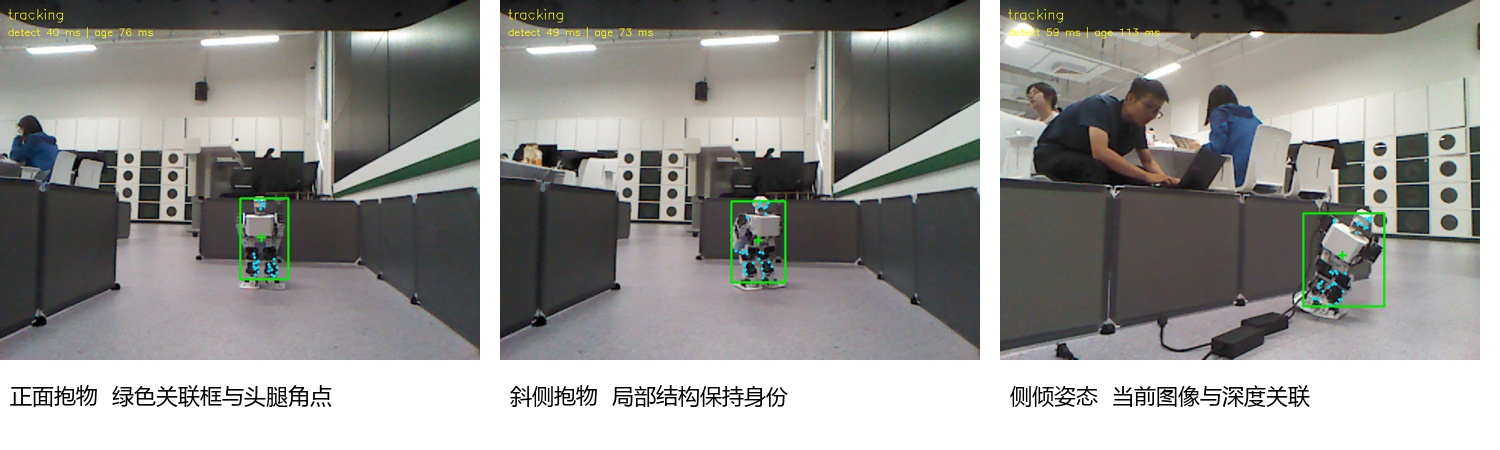
\includegraphics[width=.96\linewidth,height=.36\textheight,keepaspectratio]{figures/follow3/f3_07_poses.jpg}
\caption{实际多姿态识别输出，保留原始目标框与局部角点}\label{fig:f3-07}
\end{figure}
\Needspace{5\baselineskip}
\subsubsection{同源扰动与逐帧耗时}
以当前侧身抱红块的 12 组同步 RGB-D 样本为基础，分别施加图像平移、水平模糊、亮度衰减和随机深度缺失。平移同步处理 RGB 与深度，深度插值使用最近邻；缺失实验使用固定随机种子。原始样本及四种扰动共 60 次检测全部产生候选。另移除机器人本体、保留红块构造 12 次负样本，均未产生机器人候选。\cite{f3-jitter}

\begin{figure}[!htbp]
\centering
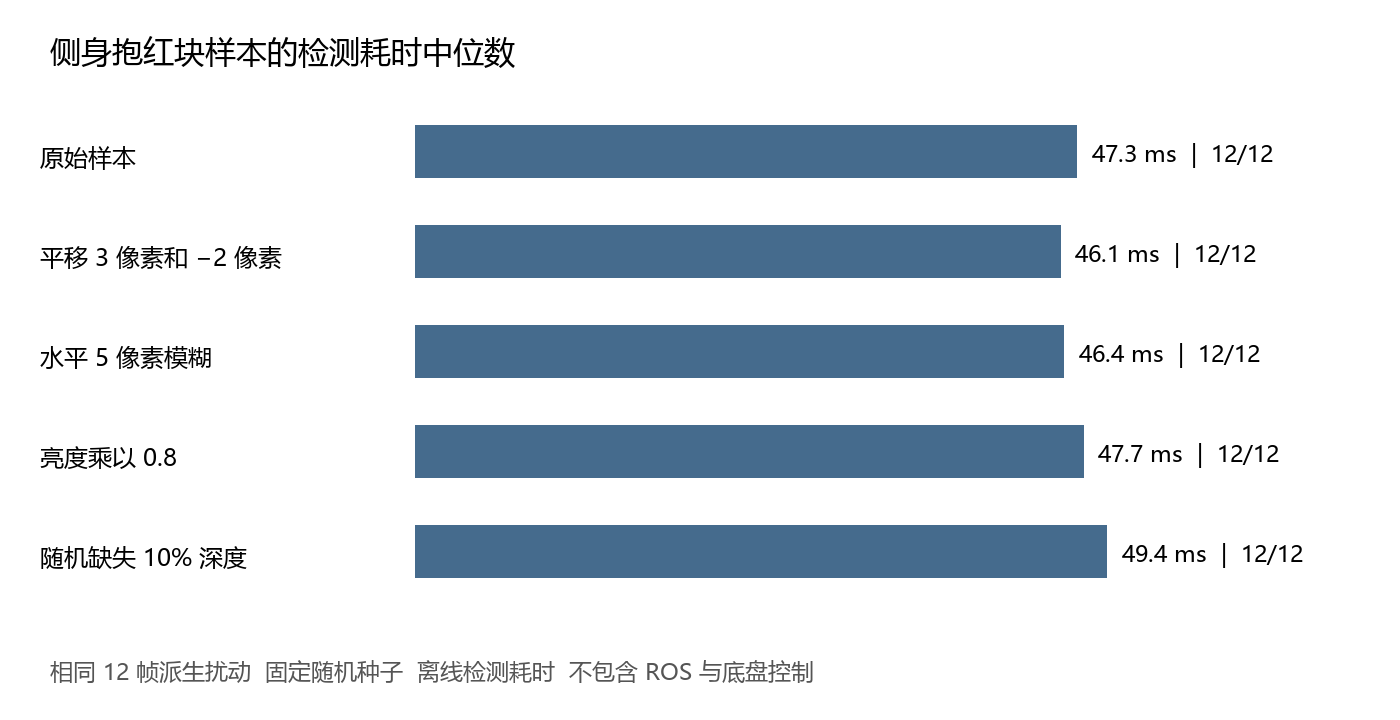
\includegraphics[width=.96\linewidth,height=.36\textheight,keepaspectratio]{figures/follow3/f3_03_jitter.png}
\caption{派生扰动回放中的检测耗时与检出次数}\label{fig:f3-03}
\end{figure}

12 帧经多种处理仍来自相同场景，60 次并非 60 个独立真实场景。结果支持对所设扰动的局部稳定性，同时说明红块加分依赖本体证据；不能由此计算整场比赛的精确率、召回率或泛化成功率。

在图~\ref{fig:f3-03}的中位数统计之外，图~\ref{fig:f3-08}保留12帧的原始检测耗时，包括高耗时样本。五组条件均检出12/12，红块单独负样本为0/12；这些结果共同说明局部扰动容忍性及红块证据的使用边界，不能把中位耗时当作每帧延迟，也不能据同源派生样本推定整场精确率或召回率。

\begin{figure}[!htbp]
\centering
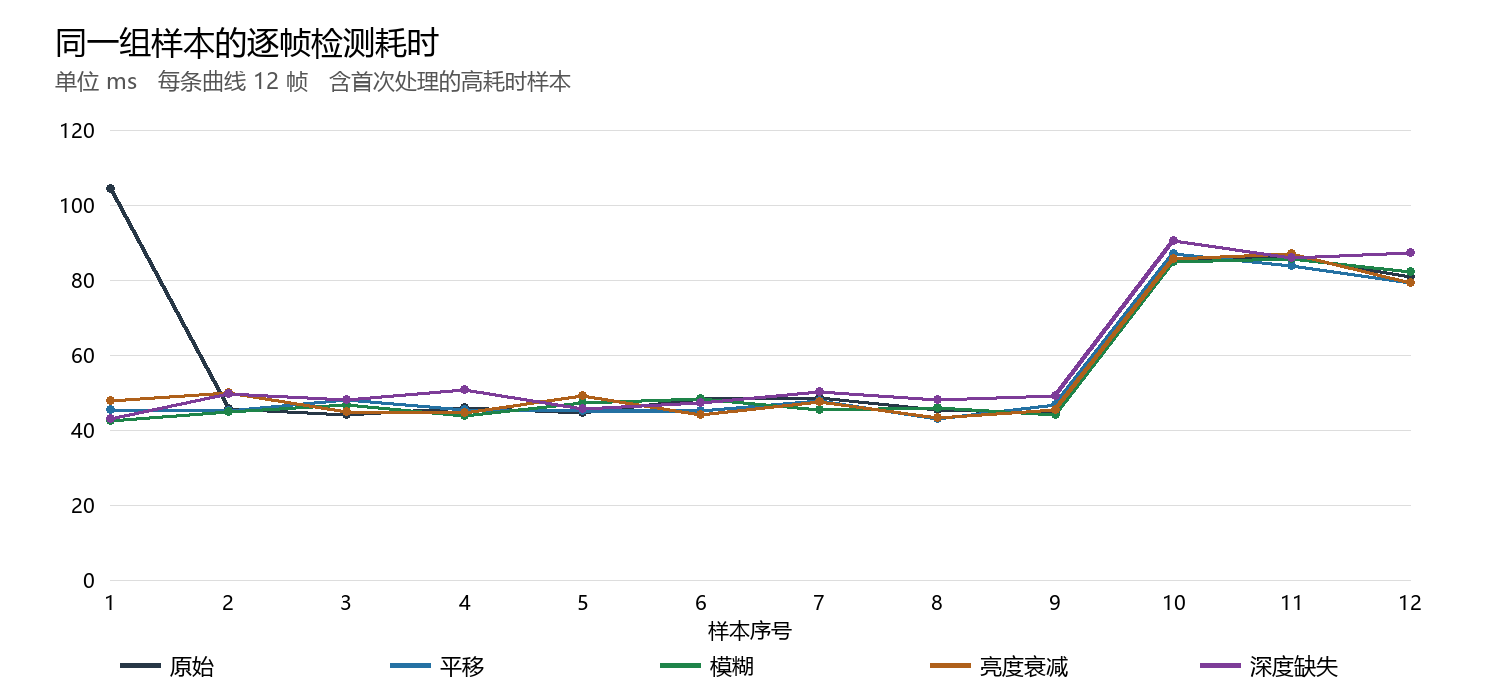
\includegraphics[width=.96\linewidth,height=.36\textheight,keepaspectratio]{figures/follow3/f3_08_frame_timing.png}
\caption{同源样本逐帧检测耗时；开发机离线测量，数据来自原始JSON记录}\label{fig:f3-08}
\end{figure}



\FloatBarrier
\Needspace{8\baselineskip}
\subsection{地图诊断与正式比赛}\label{sec:f3-field-results}
\Needspace{5\baselineskip}
\subsubsection{点云新鲜度与占据更新}
\begin{table}[!htbp]
\centering\small
\caption{地图维护诊断窗口结果}\label{tab:f3-map}
\begin{tabularx}{\linewidth}{p{.30\linewidth}p{.25\linewidth}Y}\toprule
记录项目 & 结果 & 对应含义\\
\midrule
初次现场点云年龄 P95 & 约 23 ms & 输入新鲜度正常\\
时序层后点云年龄 P95 & 约 21 ms & 仍使用当前观测\\
局部与全局地图计算频率 & 约 20 / 10 Hz & 内部占据更新\\
地图对外发布频率 & 约 7.9 / 4.1 Hz & 与 RViz 显示相关\\
10 s 内过期体素数 & 局部 474  全局 1575 & 历史证据按时释放\\
\bottomrule\end{tabularx}
\end{table}

这些数据来自 2026 年 10 月 12 日现场诊断窗口。\cite{f3-temporal} 它说明“窗口看起来不更新”需要区分传感器、占据计算、对外发布和历史证据保留。改进后无需依靠反复重启地图来释放这类旧证据。该窗口过期数属于当时场景，不能作为所有环境的固定清障性能。
\Needspace{5\baselineskip}
\subsubsection{识别与地图的同屏诊断}
图~\ref{fig:f3-05} 使用现场保留的虚拟机原始程序截图，裁去大面积空白桌面，同时保留状态终端、目标预览和 RViz。同屏可见 TonyPi 的绿色关联框，以及挡板和机器人对应的三维点与地图。RGB 图像提供身份与外观线索，深度几何提供障碍位置和可通行空间信息。

\begin{figure}[!htbp]
\centering
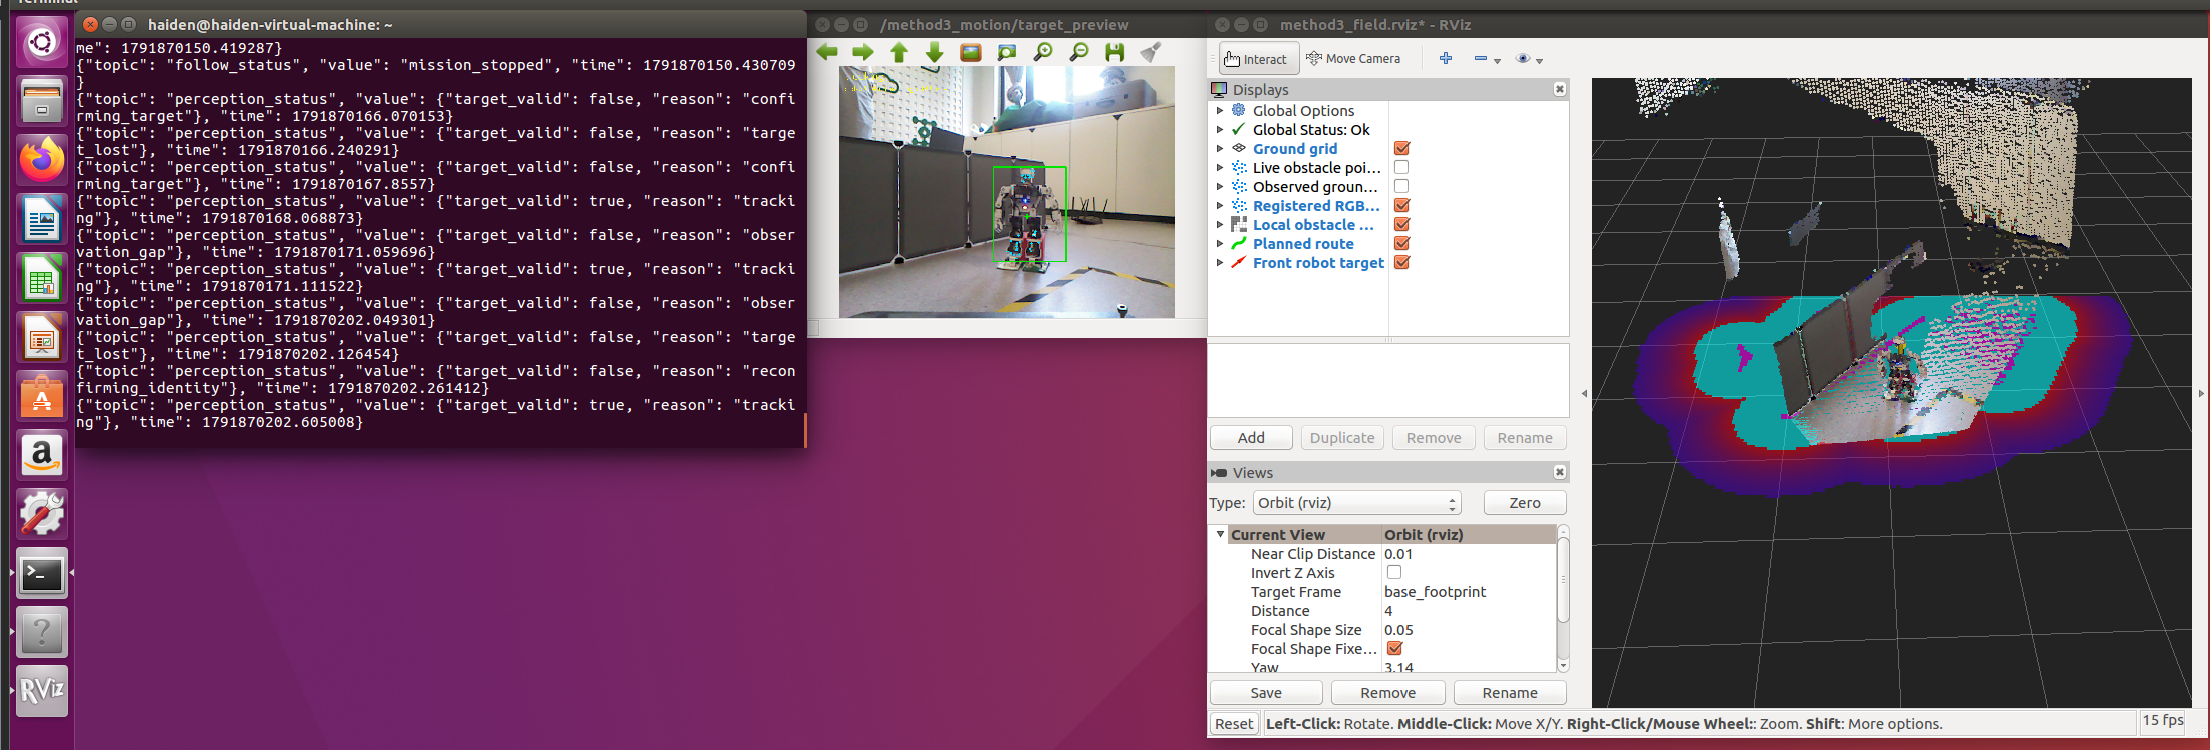
\includegraphics[width=.96\linewidth,height=.42\textheight,keepaspectratio]{figures/follow3/f3_05_program.png}
\caption{现场识别、状态终端与点云同屏；原始截图仅裁切空白桌面}\label{fig:f3-05}
\end{figure}

图~\ref{fig:f3-06} 从另一张原始程序截图中裁出 RViz 窗口。三维点云展示可见表面，地面彩色区域展示占据代价与膨胀范围，曲线和目标显示用于辅助规划诊断。历史截图也记录了目标丢失或低速重试等状态，因此这些图用于说明可视化与调试能力，比赛完成结论仍由比赛记录支持。

\begin{figure}[!htbp]
\centering
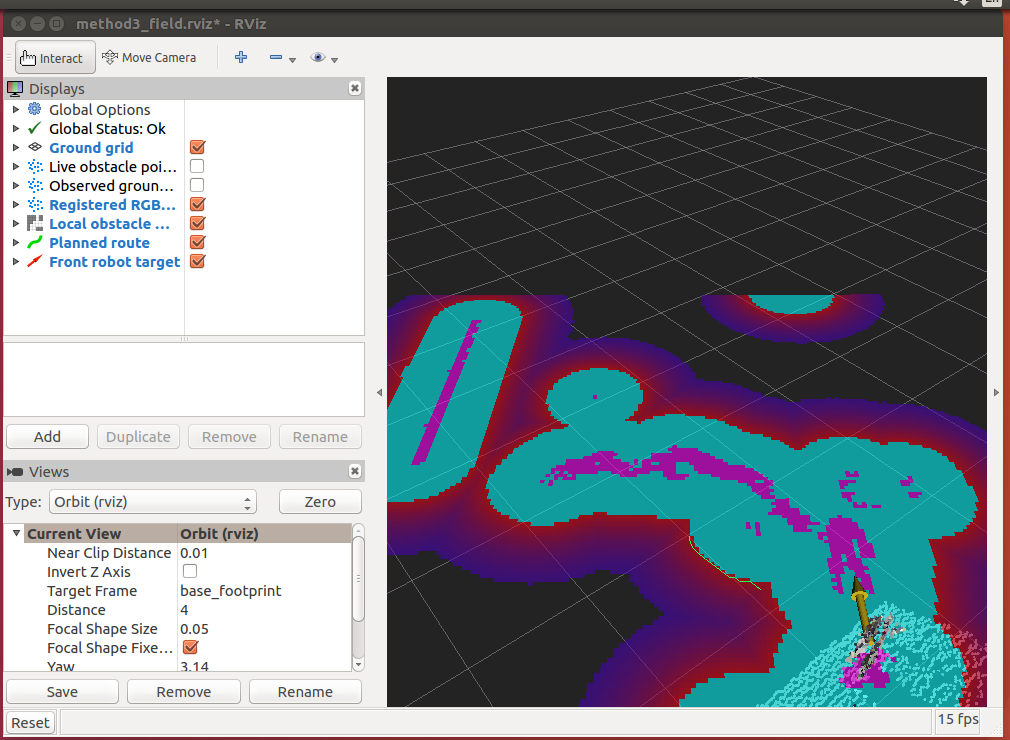
\includegraphics[width=.96\linewidth,height=.42\textheight,keepaspectratio]{figures/follow3/f3_06_rviz.png}
\caption{RViz点云与代价地图；图层颜色以运行配置为准}\label{fig:f3-06}
\end{figure}
\Needspace{5\baselineskip}
\subsubsection{比赛过程与计时结果}
本次比赛在图~\ref{fig:f3-01} 所示挡板场地完成，正式比赛耗时为 180 秒。所依据的比赛视频长 184.81 秒，拍摄到 TonyPi 抱持红色方块行进、后方多台移动机器人排队跟随及转弯区运行画面，并包含终端与 RViz 画面。正式比赛完成结果由现场确认，视频为过程佐证；两种时间采用各自口径。

\begin{figure}[!htbp]
\centering
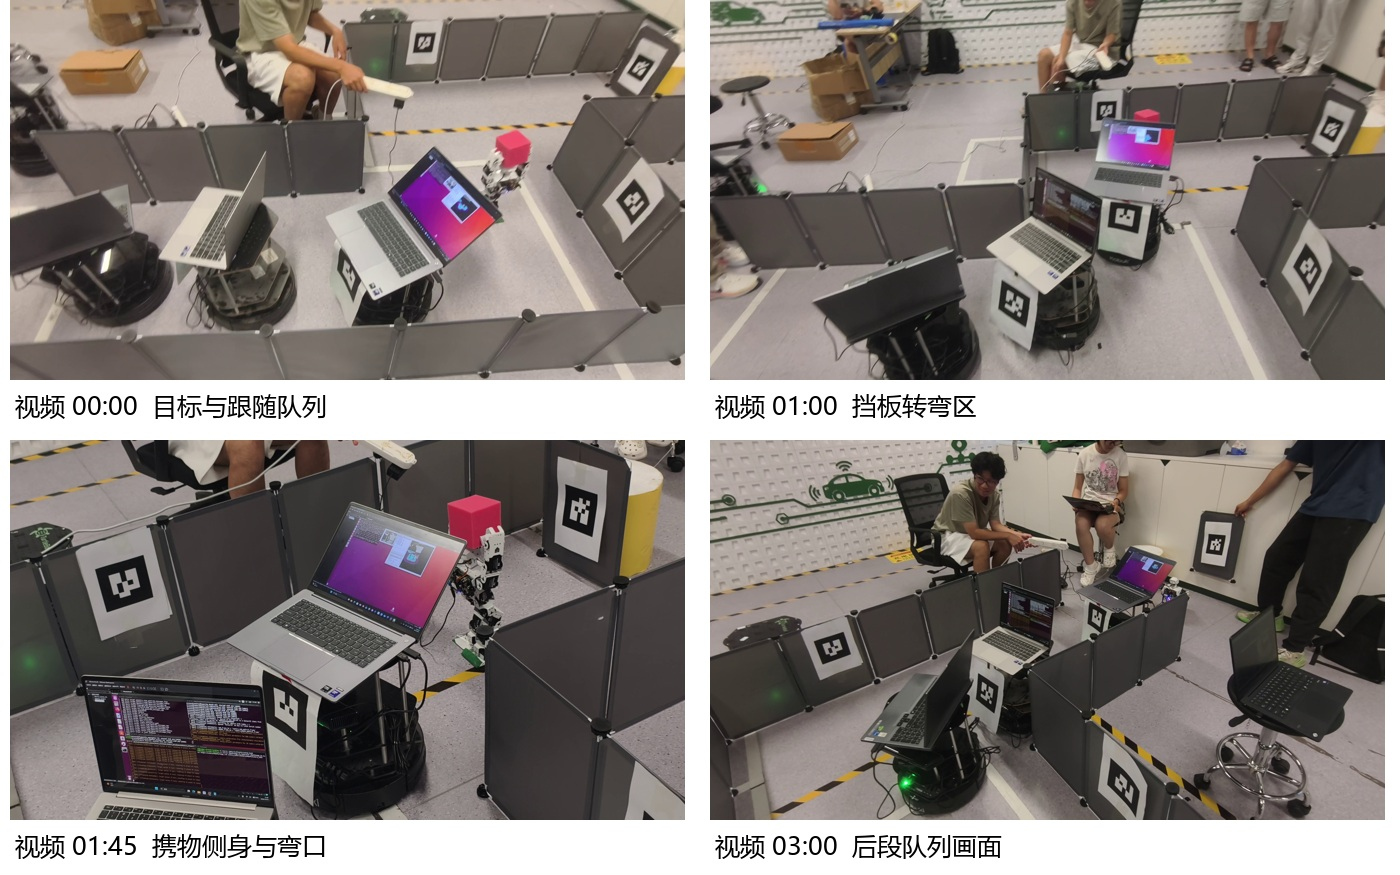
\includegraphics[width=.96\linewidth,height=.36\textheight,keepaspectratio]{figures/follow3/f3_04_race_frames.jpg}
\caption{比赛过程关键帧；图内时间为录像时间，与正式计时起止不完全相同}\label{fig:f3-04}
\end{figure}



\FloatBarrier
\Needspace{8\baselineskip}
\subsection{合成弯道规划回放}\label{sec:f3-planner-replay}
为说明“先远离目标再接近”的必要性，我们直接调用本项目 \code{reachable_standoff} 与 \code{DetourRoute}，在合成 U 形障碍中逐次生成可达子目标，并沿重建栅格路径推进几何位置。后车从开口朝后的局部死角出发，直指前车的连线被挡板截断，规划必须先退出，再沿连通空间绕至障碍侧方。

\begin{figure}[!htbp]
\centering
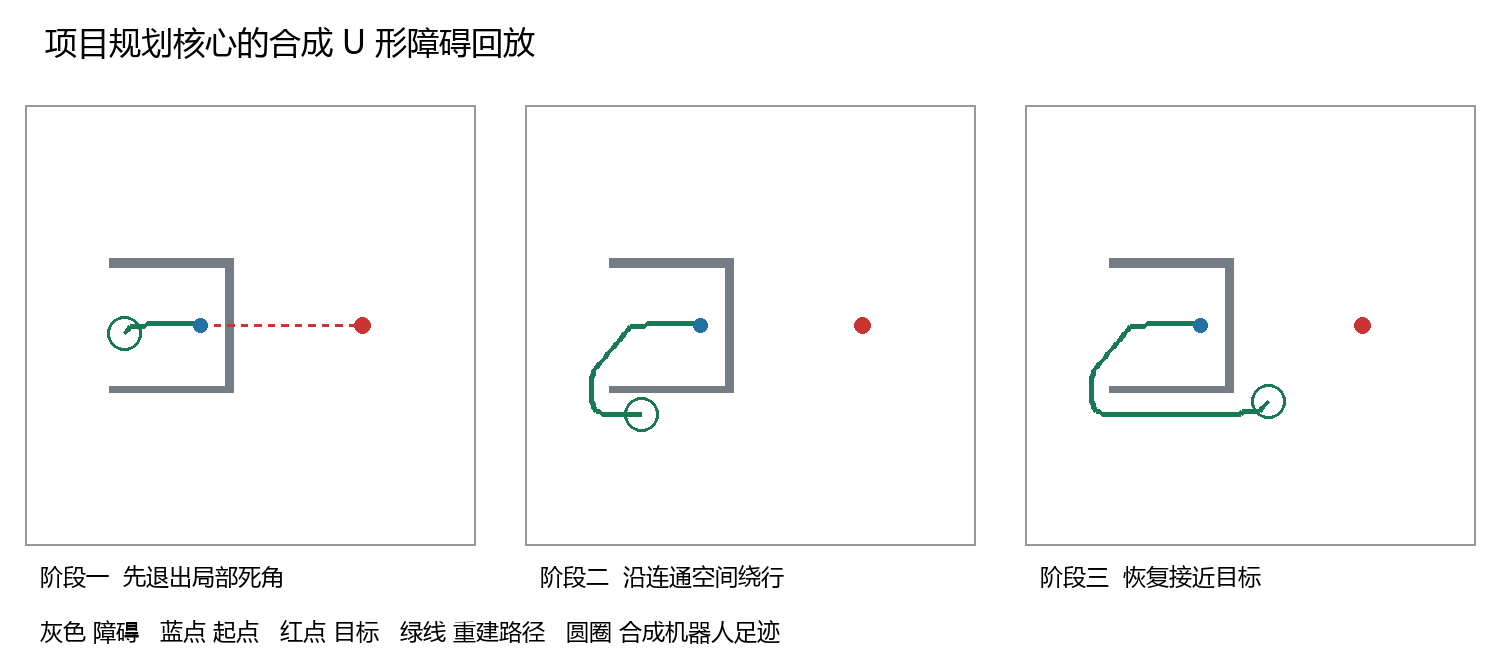
\includegraphics[width=.96\linewidth,height=.36\textheight,keepaspectratio]{figures/follow3/f3_09_planner.png}
\caption{项目规划函数的三阶段几何回放；合成栅格，非比赛地图}\label{fig:f3-09}
\end{figure}

回放使用 0.02 m 栅格和 0.12 m 的合成足迹半径，此半径仅用于算法演示，不是实车尺寸。8 次子目标更新后走出死角，目标距离由 1.15 m 先增加至约 1.98 m，再降至约 0.81 m；图~\ref{fig:f3-10} 记录这一非单调变化。若要求每一步都缩短目标距离，第一阶段的有效退出路径就会被拒绝。

\begin{figure}[!htbp]
\centering
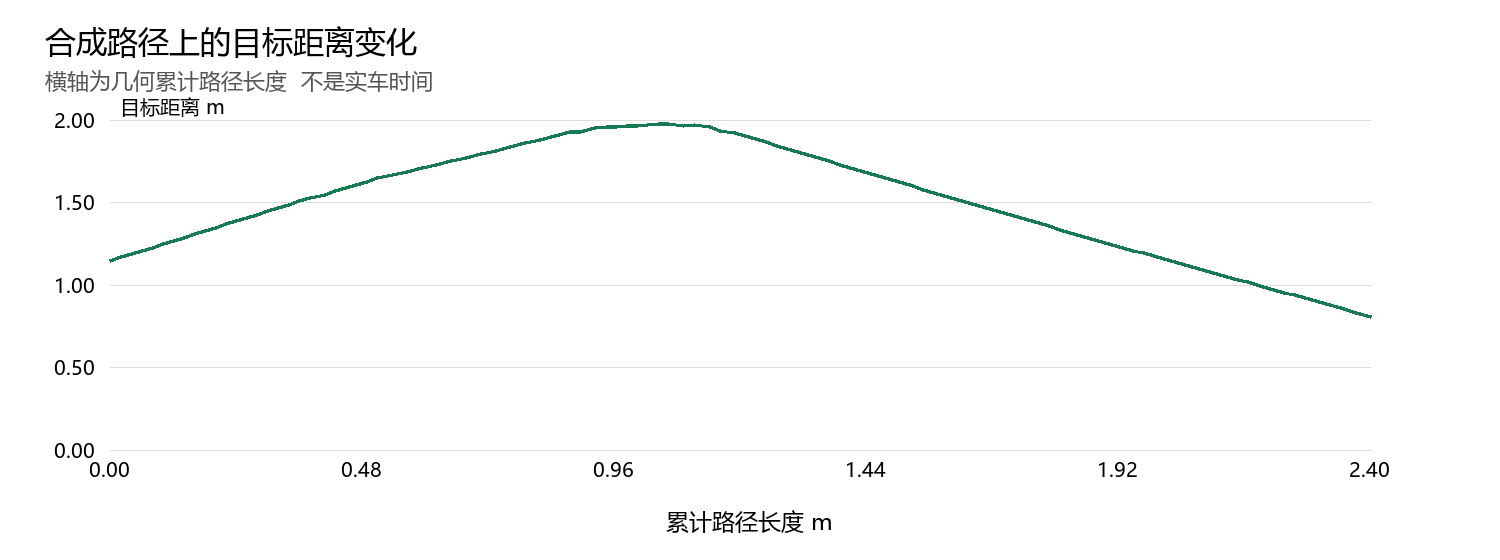
\includegraphics[width=.96\linewidth,height=.36\textheight,keepaspectratio]{figures/follow3/f3_10_planner_distance.png}
\caption{合成回放的目标距离与累计路径长度  从实际重建路径计算}\label{fig:f3-10}
\end{figure}

演示覆盖可达点选择、足迹检查和绕行路径连续性；它没有模拟 DWA 速度、轮胎动力学、传感器噪声或目标遮挡，也未推进到最终跟随停车点。正式实车仍由 Navfn、DWA 和门控执行。回放数据单独归档，便于复现算法解释，不能替代比赛结果。


\FloatBarrier
\Needspace{8\baselineskip}
\subsection{Turtlebot目标扩展验证}\label{sec:f3-extension}
除正式比赛采用的 TonyPi 目标外，开发阶段还实现了以前方 Turtlebot 为目标的视觉跟随模式。该模式用于验证目标识别的可扩展性及共用导航链路，未用于本次正式比赛；本节结果不计入 180 秒的比赛表现。

\Needspace{4\baselineskip}
\subsubsection{底盘外观与空间结构适配}

Turtlebot 的低矮黑色底盘、层板和支柱与 TonyPi 的头腿结构不同，且黑色表面可能产生深度空洞。系统为其保存独立的底盘外观参考与 RGB 模板，结合实测深度和物理宽度筛选候选；上方平台和空隙提供辅助结构证据。重叠候选抑制加入实测宽度一致性，降低局部小框压制完整底盘框的情况。仅使用结构或颜色不足以确认身份时，仍由时序关联处理歧义。

\Needspace{4\baselineskip}
\subsubsection{共用导航与独立配置}

使用场地入口参数 \texttt{--target turtlebot} 切换独立配置，\texttt{--target tonypi} 切回比赛目标。两者共用本车 RGB-D、odom 关联、滚动代价地图、可达跟随点及 Navfn/DWA 控制链路；TonyPi 的头腿角点和红块证据只在对应目标分支启用。前后车无需广播位姿，切换识别目标不意味着本节采用了另一套通信编队算法。

\begin{figure}[!htbp]
\centering
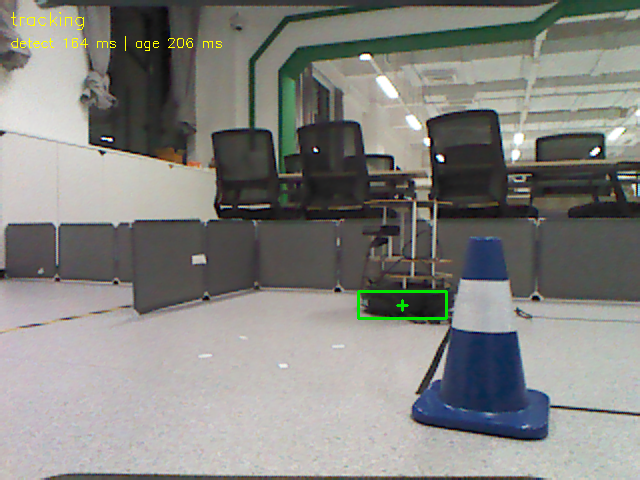
\includegraphics[width=.96\linewidth,height=.42\textheight,keepaspectratio]{figures/follow3/f3_11_turtlebot.png}
\caption{开发阶段Turtlebot目标识别输出；绿色框为已关联底盘目标}\label{fig:f3-11}
\end{figure}

\Needspace{4\baselineskip}
\subsubsection{开发回归结果与适用范围}

在一组用于调参的 12 帧正面开发回归中，输出均保留单个主要底盘框，横向中心最大相邻跳变由约 9.34 cm 降至 1.55 cm。另采约 30$^{\circ}$转角的 12 帧，新旧模板配置都保留单个真车框。这些结果说明对应开发样本的定位稳定性及目标保留情况；它们不是独立盲测，也未构成该模式的完整移动赛道验收。\cite{f3-turtlebot}


\FloatBarrier
\Needspace{8\baselineskip}
\subsection{工程讨论与结论}\label{sec:f3-discussion}
\Needspace{5\baselineskip}
\subsubsection{感知与运动的闭环耦合}
本实验的核心难点在于感知与控制互相影响。侧身漏检会使跟随目标失效；目标重新出现时需要恢复关联与导航。若规划选择使前车离开视野的绕行点，检测还会进一步变差。我们通过头腿局部证据、深度一致的红块加分、短时光流接续和视野约束，让识别结果能够持续服务规划，再通过可达跟随点和控制状态消解“有框却不走”的问题。
\Needspace{5\baselineskip}
\subsubsection{用观测证据定位停滞原因}
旧点云残影曾被直观理解为计算资源不足，但实际点云年龄只有几十毫秒。对比新点云时间戳和历史体素后，问题定位到占据证据生命周期，最终通过时序地图处理。这个过程体现了日志诊断的重要性：增加线程或降低阈值未必解决根因，必须把输入新鲜度、坐标变换、地图状态与规划拒绝原因逐层对应。

规划器、门控和底盘转发器若采用不同速度上限或转向许可，会产生规划可行但实际执行被拒的冲突。小角速度、短跟随子目标和持续回正也可能让底盘停留在起步能力边缘。场地入口统一生成限速配置，并根据里程计与状态区分到距、目标丢失、地图阻塞和无进展，减少相同问题反复出现。
\Needspace{5\baselineskip}
\subsubsection{评价范围与后续改进}
正式比赛完成验证了这套系统在本次场地与目标条件下的可用性；目前模块实验以短片段和小样本为主，后续应增加独立姿态、光照、遮挡比例与速度条件。建议用人工标注视频统计误检和漏检，用带源时间戳的 rosbag 绘制目标距离、速度、地图年龄与状态时间线，并对同一弯道重复运行统计停顿时间及重规划次数。

旧 Kinect 和 USB 虚拟化链路仍是长时运行的重要约束。软件可处理短时异常和恢复，但采集链路不稳定会直接减少有效信息。后续可通过更稳定的供电、USB 直连或原生 Linux 环境降低此类干扰，再评估更高速度与更复杂障碍布局。
\Needspace{5\baselineskip}
\subsubsection{本方式结论}
本组实现了从 RGB-D 目标识别、时序身份关联、深度障碍地图到路径规划和差速底盘执行的完整方式三链路，并在室内挡板赛道完成了比赛，耗时 3 分钟。工作的主要贡献是针对携物与侧身姿态构建互补识别证据，用有限光流维持短时连续性，并通过地图证据更新与规划控制一致性处理弯道停滞。现场采样、扰动回放和比赛过程共同支撑了系统在本实验条件下的跟随与避障能力。



\FloatBarrier
\Needspace{8\baselineskip}
\subsection{实现索引与数据来源}\label{sec:f3-reproduction}
\begin{table}[!htbp]
\centering\small
\caption{方式三关键代码与实现位置}\label{tab:f3-code}
\begin{tabularx}{\linewidth}{p{.20\linewidth}Y}\toprule
功能 & 仓库路径\\
\midrule
场地启动 & \code{tools/start_method3_field.sh}\newline \code{tools/run_rgbd_field_session.py}\\
RGB-D 检测节点 & \code{turtlebot/follow3/rgbd_following/scripts/rgbd_target.py}\\
身体与抱物特征 & \code{src/rgbd_following_core/body.py}\newline \code{src/rgbd_following_core/tonypi_parts.py}\\
跟踪与光流 & \code{src/rgbd_following_core/tracking.py}\newline \code{src/rgbd_following_core/feature_flow.py}\\
跟随与规划 & \code{scripts/rgbd_follower.py}\newline \code{src/rgbd_following_core/planning.py}\\
地图更新 & \code{scripts/rgbd_obstacles.py}\newline \code{src/temporal_voxel_layer.cpp}\\
导航与速度门控 & \code{config/navigation.yaml}\newline \code{scripts/rgbd_velocity_gate.py}\\
\bottomrule\end{tabularx}
\end{table}

表中 src、scripts、config 的相对路径均以 \code{turtlebot/follow3/rgbd_following} 为基准。报告对应仓库中场地迭代后的实现；通用示例配置、历史调试轮次和正式比赛配置应区分。

\Needspace{4\baselineskip}
\FloatBarrier

采样频率、跟踪状态与光流补接记录对应抱物采样和系统优化文档\cite{f3-carry,f3-opt}，地图更新指标对应2026年10月12日诊断记录\cite{f3-temporal}。扰动实验原始记录为\code{.tools/system_audit/red_carry_jitter_results.json}及\code{validate_red_carry_jitter.py}，本地副本与合成规划数据分别归档为\code{data/follow3/recognition_evidence.json}、\code{planner_demo_evidence.json}。\cite{f3-jitter}

比赛过程以《机器人比赛一.mp4》、场地原图\code{IMG_20261013_160409.jpg}及现场确认结果为依据；当前交付包保存关键帧和视频元数据，未重复包含原视频。\cite{f3-race} Turtlebot目标的开发回归记录另见对应诊断文档。\cite{f3-turtlebot} 相关路径及文献统一列于报告末尾的参考资料中，便于区分源码、模块数据和比赛证据。



\FloatBarrier

\Needspace{25\baselineskip}

\subsection{成员职责与协作分工}

本组由何奇涛、李雨翰、林子昂和陈韦诺四人组成，按感知、识别跟踪、地图规划和控制集成四个核心模块均衡安排工作量，每人占25\%。每人承担所负责模块的实现、测试和对应报告撰写；实车联调、数据复核、视频整理与报告统稿由四人共同完成。以下为职责分工安排，实际交付由成员共同核对，学号另行补充。
\begin{table}[!htbp]\centering\small
\caption{方式三四人成员职责与协作分工}\label{tab:f3-members}
\begin{tabularx}{\linewidth}{p{18mm}YY}\toprule
姓名 & 核心职责 & 模块交付与共同协作\\\midrule
何奇涛 & RGB-D感知与候选提取：图像同步、配准核对、深度测距及目标候选筛选。 & 感知配置与输入诊断记录、候选检测测试及对应文稿；共同参与实车联调与数据复核。\\
李雨翰 & 身份识别与连续跟踪：外观模板、头腿与红块特征、时序关联及短时光流补接。 & 身份与跟踪配置、多姿态及遮挡测试、鲁棒性图表及对应文稿；共同参与实验与报告复核。\\
林子昂 & 障碍地图与路径规划：障碍点云、时序占据更新、滚动代价地图及可达跟随点选择。 & 地图与规划配置、绕障回放和弯道测试记录及对应文稿；共同参与现场联调与结果分析。\\
陈韦诺 & 运动控制与系统集成：Navfn/DWA对接、速度门控、场地启动和终点停车逻辑。 & 控制与启动配置、异常恢复和完整链路测试记录及对应文稿；共同参与视频整理与报告统稿。\\\bottomrule
\end{tabularx}\end{table}

\FloatBarrier

\endgroup
